\documentclass[a4paper, 12pt]{article}

\usepackage{hyperref}
\usepackage{fullpage}
\usepackage[top=0.5in, bottom=1.5in, left=0.5in, right=0.5in, footskip=4em]{geometry}
\usepackage{amsmath}
\usepackage{fancyhdr}
\usepackage[usenames,dvipsnames]{xcolor}
\usepackage{pgfornament}

\usepackage[shortlabels]{enumitem}
\usepackage{xspace}
\usepackage{lastpage}
\usepackage{multicol}
\usepackage{blindtext}
\usepackage{titling}
\usepackage{standalone}
\usepackage{amsfonts}
\usepackage[framemethod=TikZ]{mdframed}
\usetikzlibrary{calc}
\usepackage{lineno}
\usepackage{amsthm}
\usepackage{amssymb}
\usepackage{mathtools}
\usepackage{datetime}
\usepackage[most]{tcolorbox}
\usepackage{cancel}
\usetikzlibrary{tikzmark}
\linenumbers


%BEGIN_FOLD Commands
\newcommand{\half}{\frac{1}{2}}
\newcommand{\epv}[1]{\ensuremath{\left< #1 \right>}\xspace}
\newcommand{\variance}{\ensuremath{\text{Var}}}
\newcommand{\eout}{\ensuremath{E_\text{out}}\xspace}
\newcommand{\ein}{\ensuremath{E_\text{in}}\xspace}
\newcommand{\cx}{\ensuremath{\mathcal{X}}\xspace}
\newcommand{\cz}{\ensuremath{\mathcal{Z}}\xspace}
\newcommand{\real}{\mathbb{R}}
\DeclareSymbolFont{extraup}{U}{zavm}{m}{n}
\DeclareMathSymbol{\varheart}{\mathalpha}{extraup}{86}
\DeclareMathSymbol{\vardiamond}{\mathalpha}{extraup}{87}
\renewcommand{\heartsuit}{\textcolor{red}{\varheart}}
\renewcommand{\diamondsuit}{\textcolor{red}{\vardiamond}}
\newcommand{\definition}{\vspace{1em}\noindent\textbf{Def:} }
\newcommand{\theorem}{\vspace{1em}\noindent\textbf{Theorem:} }
\newcommand{\predicate}{\vspace{0.25em}\noindent\textbf{Inductive Predicate:} }
\newcommand{\inductivestep}{\vspace{0.25em}\noindent\textbf{Inductive Step:} }
\renewcommand{\proof}{\vspace{0.5em}\noindent\textbf{Proof:} }
\newcommand{\lemma}{\vspace{1em}\noindent\textbf{Lemma:} }
\newcommand{\hint}{\textbf{Hint:} }
\newcommand{\basecase}{\vspace{0.25em}\noindent\textbf{Base Case:} }
\newcommand{\inductivehypothesis}{\vspace{0.25em}\noindent\textbf{Inductive Hypothesis:} }
\newcommand{\collorary}{\vspace{1em}\noindent\textbf{Collorary:} }
\newcommand{\qedd}{\qed\newline}
\newcommand{\kwd}[1]{\textcolor{blue}{\textbf{\underline{#1}}}}
\newcommand\ColorBox[2][]{%
	\stepcounter{mybox}%
	\node[draw=red!70!black,fill=red!20,align=left,#1] (box\themybox) {#2};
}
\newcommand{\expl}[2]{%
	\underset{\substack{\uparrow\\\mathrlap{\text{\hspace{-1em}#2}}}}{#1}}
\newcommand{\uexpl}[2]{%
	\overset{\substack{\mathrlap{\text{\hspace{-1em}#2}}\\\downarrow}}{#1}}
\newcommand{\st}{\text{ such that }}
\newcommand{\R}{\textcolor{red}{R}}
%\newcommand{\qed}{\ensuremath{\blacksquare}}
%END_FOLD
\newcommand{\sidenote}[1]{\textcolor{gray}{#1}}

%BEGIN_FOLD miscellaneious default
\makeatletter
% Make a copy of macros responsible for entering display math mode
\let\start@align@nopar\start@align
\let\start@gather@nopar\start@gather
\let\start@multline@nopar\start@multline
% Add the "empty line" command to the macros
\long\def\start@align{\par\start@align@nopar}
\long\def\start@gather{\par\start@gather@nopar}
\long\def\start@multline{\par\start@multline@nopar}
\makeatother
\setlength{\columnsep}{1cm}
%opening
\setlength{\abovedisplayskip}{-\baselineskip}%
\setlength{\abovedisplayshortskip}{\abovedisplayskip}%

\pagestyle{fancy}
\renewcommand{\headrulewidth}{0pt}
\lfoot{\small{\course}: Week \weekno}
\rfoot{\small{\thetitle}}
\rhead{}
\cfoot{\pgfornament[height=1em, ydelta=-0.4em]{17} \thepage of \pageref{LastPage}  \pgfornament[height=1em, ydelta=-0.4em]{18}}

\DeclareMathOperator{\sign}{sign}
\newcommand{\vect}[1]{\ensuremath{\mathbf{#1}}\xspace}

\tikzstyle{every picture}+=[remember picture]
\newcommand{\bwgrid}[1]{
	\def \aaa #1
	
	\foreach \y in {0,1,2} {
		\foreach \x in {0,1,2} {
			\pgfmathsetmacro{\clr}{\aaa[\x][\y]}
			%\message{aaa \clr}
			\definecolor{MyColor}{rgb}{\clr,\clr,\clr}
			\path[fill=MyColor] (\x,\y) rectangle ++(1,1); 
		}
	}
	\draw[step=1cm,very thin] (0,0) grid (3,3);	
}

\setenumerate{label=\alph*.)}
\definecolor{db}{RGB}{100,65,23}
\newtheoremstyle{examplestyle}% name
{}%         Space above, empty = `usual value'
{}%         Space below
{}% Body font
{}%         Indent amount (empty = no indent, \parindent = para indent)
{}% Thm head font
{}%        Punctuation after thm head
{\newline}% Space after thm head: \newline = linebreak
{\textbf{\textcolor{db}{\thmname{#1}\thmnumber{ #2}:} \thmnote{ #3}}}%         Thm head spec
\theoremstyle{examplestyle}

\newtheorem{examplethm}{Example}
\newenvironment{example}[1][]{\begin{mdframed}[style=example]\begin{examplethm}[#1]}{\end{examplethm}\end{mdframed}}

\newenvironment{example*}[1][]{\begin{mdframed}[style=example]\begin{examplethm}[#1]\end{examplethm}}{\end{mdframed}}
\newenvironment{Figure}
{\par\medskip\noindent\minipage{\linewidth}}
{\endminipage\par\medskip}
\newenvironment{formula}{
	\begin{mdframed}[style=formula]
	}{
\end{mdframed}}
%END_FOLD

\newcommand{\course}{Discrete Math}
\title{State Machine and Invariant}
\newcommand{\weekno}{2}

\begin{document}
\begin{center}
	\textcolor{orange}{\textsc{\course}}\\
	\huge\textbf{\textsc{\thetitle}}\\
	\small\textcolor{gray}{Last updated:\, \today \, \currenttime}\\
	\pgfornament[width=0.7\textwidth, color=white!30!black]{88}
\end{center}

\begin{multicols}{2}
Invariant is a very concept in computer science. It is an essential tool in proving program correctness. Let us explore the concept of invariant through examples.

\section*{Chessboard}

\includestandalone[width=0.8\linewidth]{chess}

First let us consider a bishop from chess game. For simplicity, let us assume that the board is infinite. Bishop can only move diagonally. It does not take too long for us to realize that if the bishop start in a black square then it will always end up in a black square no matter how many times you move.

This is the concept of \kwd{invariant}. It is something that does not change no matter how you pick \kwd{transition} from the current \kwd{state} to the next.

The last sentence contains so many keywords. So, let us define them before we go on and actually write a formal proof that bishop starting in a black square cannot go to white square.

\definition A \kwd{state} is just a configuration of the problem.

For example, for the bishop problem we are dealing with each configuration is defined by just where the bishop each. This can be simply defined by two number $(x,y)$. For instance, $(5,3)$ represents the state that the bishop is at $x=5$ and $y=3$.

\definition A \kwd{transition} is a function that take in one state and return another state.

For our purpose, it is the moves. For example, since we are only allowed to move diagonally the moves are
\begin{enumerate}
	\item North East: that is $(x,y) \to (x+1, y+1)$.
	\item North West: $(x,y) \to (x-1, y+1)$.
	\item South East: $(x,y) \to (x+1, y-1)$.
	\item South West: $(x,y) \to (x-1, y-1)$.
\end{enumerate}
For example, the NorthEast($(5,3)$) = $(6,4)$.

\definition The set of states along with transitions is call a \kwd{State Machine} $M = (S, T)$. For our purpose, it just all the possible configurations along with the valid moves.


\definition A \kwd{reachable} states of a state machine $M$ are defined recursively as
\begin{itemize}
	\item The start state is reachable.
	\item If state $p$ is reachable state and $p \to q$ is a transition of $M$ then $q$ is also a reachable state of $M$.
\end{itemize}

\definition A \kwd{preserved invariant} of a state machine is a predicate $I$, on states, such that whenever $I(q)$ is true for state $q$ and $q\to r$ is a valid transition then $I(r)$ holds.

For example, our invariant must have something to do with landing on black square. Using our state notation we defined, the black square is defined as $x+y$ is even. Thus, our preserved invariant is
\begin{center}
	$I((x,y)):= x+y$ is even.
\end{center}
We will prove this.

Note that for the preserved invariant, we only care that it propagate when it is true. We do not care when $I$ returns false whether it will propagate along the transitions or not.

\lemma $I((x,y)):= x+y$ is even is a perserved invariant for our bishop state machine. 

\proof All we need to show is that if $I(a,b)$ is true for some $a,b$ then for every possible transition($T$), $I(T(a,b))$ is also true.

So, since $I(a,b)$ is true. That means
\[
	a+b \text{ is even.}
\]

Then we need to show are
\begin{itemize}
	\item North-East: $NE(x,y) = (x+1, y+1)$. We need to show that $NE(a,b)$ still make $I$ true. That is we need to show that $(a+1)+(b+1)=a+b+2$ is even.
	
	Since $a+b$ is even, $a+b+2$ is even.\checkmark
	\item North West: $NW(x,y) = (x-1,y+1)$.
	
	Since $a+b$ is even, $a-1+b+1 = a+b$ is even of course.\checkmark
	\item The other two cases for South West and South East is left for the read as an exercise.
\end{itemize}
Since we have shown that $I$ is preserved through all possible transitions. $I$ is a preserved invariant.\qedd

Now let us show that if we start in a black square then we will always end up in a black square. For your homework you don't need to show this. All you need to do is to show that a predicate is a preserved invariant and that you start in a correct state. Then you can just use the result of the proof below.

\theorem If we start in a state where $I(start)$ is true, then $I(u)$ for all reachable states($u$).

\proof The proof is induction on the number of transitions.

\predicate $P(s):=$ if $q$ is a state reachable in $s$ transitions, then $I(q)$ (is true).

\basecase $P(0)$ is true since it is where we start and it is a black square and by definition $x+y$ for black square is even.\checkmark

\inductivestep

\inductivehypothesis Let us assume that at step that $P(k)$ is true that is all state reachable in $k$ steps is black($I(q)$ is true).

We want to show that all states reachable in $k+1$ steps is also black.

With out loss of generality let the state reachable in $k+1$ step be $r$. Since $r$ is reachable in $k+1$ step, there must exists two things
\begin{enumerate}[1)]
	\item State $q$ that is reachable in $n$ step.
	\item A transition $q\to r$.
\end{enumerate}

First, since $q$ is a reachable in $n$ step, by IH, $I(q)$ is true. Second, since $I$ is a preserved invariant by lemma above and there exists a transition $q \to r$ then $I(r)$ is also true.

Thus by mathematical induction, if we start in a state where $I(start)$ is true, then $I(u)$ for all reachable states($u$).\qedd

Again you don't need to show this in the homework or exam. It is just stating the obvious formally. All you need to do is to find the relavant preserved invariant and show that it is really a preserved invariant. Then you just add a sentence saying that since we start in a state that the preserved invariant is true and therefore this quantity is the same no matter how many step we make.

\section*{Tiling Dominoes}
Let us consider a problem of tiling $2\times 1$ dominoes on an $8\times 8$ grid with the opposite corners taken out.

\begin{center}
	\includestandalone[width=0.8\linewidth]{chessnocorner}
\end{center}

After a trying a couple times you will realized that this is not possible. The basic idea is that each time we place a dominoes the number of black and white left on the board both get reduced by one. Therefore, since we start with board with not equal number of white and black $(0,0)$ is not reachable. Let us show this using state machine and perserved invariant.

Let us defined the tiling as a state machine. Let us define the states to be the nubmer of black white left on the board$[b,w]$. Of course now each state represents so many possible configuration but all we care is that it gets our job done.

Let us defined also our transitions. Placing 1 $2\times1$ domino on the board will reduce the number of black and the number of white by $1$. So our transitions is $T:[b,w] \to [b-1, w-1]$.

\theorem $P:= w-b = 2$ is a preserved invariant.

\proof Let us assume that we start in state $q = [b_q, w_q]$ and that $ w_q - b_q = 2$.

We want to show that $r = T(q) = [b_r, w_r]$ satisfy $w_r - b_r = 2$.

Since $w_r = w_q -1$ and $b_r=b_q -1$,
\[
	w_r - b_r = w_q -1 - b_q +1 = w_q-b_q = 2
\]
\qedd

\collorary Since $P:=w-b=2$ is an invariant and $[0,0]$ does not satisfy the invariant. $[0,0]$ is not reachable.



\section*{Red/Black Pairs Revisit}
Let us reconsider the problem on homework 1 to show that we always get equal number of black and red pairs. A lot of you had this same idea except you lack the tools to write it properly. So, let us do it once and for all.

First, we need to define the states and transitions. The states are all the permutation of cards. However, sometime we don't need to know all the fine detail of the states. All we need to know is a permutation of the card colors. We can represent the state with a string of 26 B and 26 \R. There are so many of them (we will learn how to count that later). Here are some examples:
\begin{center}
	BB\ldots BBB\R\R \ldots \R\R\R\\
	 $\vdotswithin{=}$\\
	B\R B\R\ldots B\R B\R
\end{center}

For this example, we want to show that all permutations of cards will give us the same number of black pairs and red pairs. So, all we need to do is to show that all the permutations are \emph{reachable}. So, let consider a simple transitions of switching two adjacent cards. By a serie of switching two adjacent cards you can reach any permutation.

\lemma $I(s) = $ drawing pairs from permutation $s$ will give the same number of black pairs and red pairs at the end. $I$ is a preserved invariant.

\proof Like the previous example all we need to show that all possible moves does not change ($I$).

There are actually not many cases we need to consider.

First, if the pair we switch is already in the same pair bracket then switching them doesn't change the number of black pairs and the number of red pairs. 

Before:
\[
	\ldots BB | B\R | XY| BB \ldots
\]

After
\[
\ldots BB | B\R | YX | BB \ldots
\]

Since we start in the state that black and red pairs are equal therefore, the end state has equal number of black and red pairs.\checkmark

Second, now we need to consider the case where we switch the cards from different pair bracket. $ \ldots | WX|Y Z| \to \ldots| WY|X Z|\ldots $
\begin{enumerate}
	\item If $X$ and $Y$ has the same color then switching them doesn't do anything to the number red pairs and the number of black pairs.\checkmark
	\item If $X$ and $Y$ are of different colors, then we have couple cases.
	
	\begin{enumerate}[i)]
		\item $\ldots|B \R | B B|\ldots \to \ldots|B B | \R B|\ldots $. The number of red and black pairs remain the same. \checkmark
		\item $\ldots|R \R | B B|\ldots \to \ldots|R B | \R B|\ldots $. The number of red and black pairs both get reduced by one. Therefore the number of red and black pairs are still equal.\checkmark
		\item $\ldots|B \R | B \R|\ldots \to \ldots|BB | \R \R|\ldots $. The number of red and black pairs both get increased by one. Therefore the number of red and black pairs are still equal.\checkmark
		\item We can get all the other cases by switching what we call \R \;and what we call B.
	\end{enumerate}
	
\end{enumerate}

Since we have shown for all the transition that if the number of pairs are equal before the trasition then the number of pair will be equal after the transition. Thus, $I$ is a preserved invariant.\qedd

Now we need to show that one state has equal number of black and red pairs. Then we can use it to reach all other states. This is easy since the state of 26 consecutive black and 26 consecutive red has equal number of black and red pairs BB \ldots BB\R \R\ldots \R \R.

\collorary All permutation gives equal number of red and black pairs

\proof Since the state of 26 consecutive black and 26 consecutive red has equal number of black and red pairs. Plus, all permutation are reachable. By the preserved invariant we show in the lemma above, all permutations give the same number of black and red pairs.\qedd

\section*{The Roulette-ish.}

Roulette is a game where the house rolls a ball down a spinning wheel and see what number it lands in. Each number has a color associate with it 18 Red and 18 Blacks and there is one or two green. The bettor can bet whether the ball lands on red or black. The pay out is 2:1. This means that if you bet 1 Baht and you win, you get 2 Baht giving you 1 Baht profit. If you lose you lose you get nothing. Roulette is one of the worst game in casino\footnote{Baccarat has the best odd.}. The house has an advantage over you since there is that one/two green where the house wins both black and red bet.

Let us consider a similar game. The game consists of 5 cards: 2 red, 2 black and one joker. The red and black card represents the red and black numbers while the joker represent the green slot.

The game plays is as follow, the house shuffle the card and open one at a time until he ran out of card. The bettor tell exactly which color he is gonna bet and exactly how he is going to calculate the betting amount for each turn. As the house open one card at a time the winning/losing amount is booked and sum up at the end.

If we bet the same color with the same amount everytime, it is clear that we are goint to lose the money for sure.

Consider the following betting strategy, we will bet on red every time. But, the amount of bet will be
\begin{enumerate}
	\item The starting bet is 16 Baht.
	\item Half the previous amount if I win in the previous round.
	\item 1.5 times the previous amount if I lose in the previous round.
\end{enumerate}

Playing this a few rounds you will be convinced that you will always win the same amount of $5$ Baht everytime. Let us prove this.

Let us use the state as all the permutation of the 5 cards and the transitions a switching two adjacent cards like in the previous example.

\theorem All permutation of cards give the same winning amount.

\proof First, if the two card we switch are of the same color then it doesn't change anything.

So, we need to show that if the two cards are not the same then the net winning amount are the same.
\[
xxx\expl{|}{Begin}B\R\expl{|}{End}yyyyy \to xxx\expl{|}{Begin}\R B\expl{|}{End}yyy
\]
Since we only switch two cards, all we need to show is that
\begin{enumerate}
	\item If we begin the pair with same amount of bet then at the end of the pair we will have to bet the same amount on the turn right after the pair.
	\item We have to win/lose exactly the same amount during these two turn.
\end{enumerate}

Let us prove the first one first. If the bet entring the two turn is $b$. There are two cases
\begin{enumerate}
	\item We win then lose. Since we win on the first round, the bet on the second of the two turn is $b\times \half$. Then, we lose, therefore the bet amount on the turn right after this is $b \half \frac{3}{2}$.
	\item If we lose then win, Since we lose the bet on the first round the bet on the second round is $b \frac{3}{2}$. Then we win on the second round, therefore, the bet amount on the turn right after the pair is $b \frac{3}{2}\half$
\end{enumerate}

Since the two are equal, we got what we want for the first property. Now we are left to show that the winning/losing amount is the same before and after switching.

\begin{enumerate}
	\item We win then lose. So, for the first one we win $b$ Baht and lose $\half b$. Therefore we win the total amount of $\half b$.
	\item We lose then win. So, for the first on we lose $b$ Baht and the second round we win $\frac{3}{2} b$. Therefore, we win in total $\half b$.
\end{enumerate}
The two case give the same winning amount.

Therefore, switching the two cards has no effect on the total winning/losing amount. \qedd

Now all we need to show that it is 5 Baht is to calculate an easy one.

\section*{The 15-puzzle.}
The 15 is a puzzzle where you have 15 number arrange on a $4\times4$ grid. You can slide a number to its empty adjacent slot. 
\begin{center}
	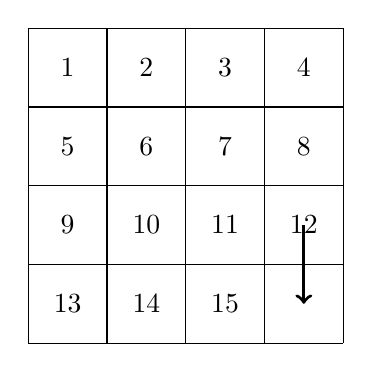
\begin{tikzpicture}
	\draw[step=1cm] (0, 0) grid (4, -4);
	\node()[anchor=center] at (0.5, -0.5) {1};
	\node()[anchor=center] at (0.5, -1.5) {5};
	\node()[anchor=center] at (0.5, -2.5) {9};
	\node()[anchor=center] at (0.5, -3.5) {13};
	\node()[anchor=center] at (1.5, -0.5) {2};
	\node()[anchor=center] at (1.5, -1.5) {6};
	\node()[anchor=center] at (1.5, -2.5) {10};
	\node()[anchor=center] at (1.5, -3.5) {14};
	\node()[anchor=center] at (2.5, -0.5) {3};
	\node()[anchor=center] at (2.5, -1.5) {7};
	\node()[anchor=center] at (2.5, -2.5) {11};
	\node()[anchor=center] at (2.5, -3.5) {15};
	\node()[anchor=center] at (3.5, -0.5) {4};
	\node()[anchor=center] at (3.5, -1.5) {8};
	\node()[anchor=center] at (3.5, -2.5) {12};
	\draw[very thick, ->] (3.5,-2.5) -- (3.5, -3.5);
	\end{tikzpicture}
\end{center}

Around 1880, Sam Loyd offer a 1000\$ prize for anyone who can solve the puzzle with 14-15 switch.

\begin{center}
	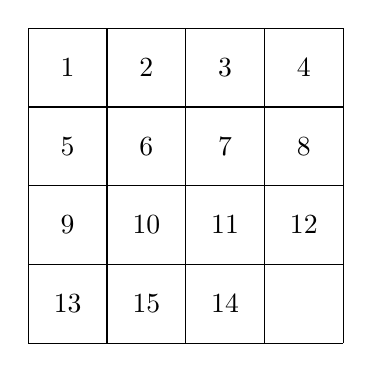
\begin{tikzpicture}
	\draw[step=1cm] (0, 0) grid (4, -4);
	\node()[anchor=center] at (0.5, -0.5) {1};
	\node()[anchor=center] at (1.5, -0.5) {2};
	\node()[anchor=center] at (2.5, -0.5) {3};
	\node()[anchor=center] at (3.5, -0.5) {4};
	\node()[anchor=center] at (0.5, -1.5) {5};
	\node()[anchor=center] at (1.5, -1.5) {6};
	\node()[anchor=center] at (2.5, -1.5) {7};
	\node()[anchor=center] at (3.5, -1.5) {8};
	\node()[anchor=center] at (0.5, -2.5) {9};
	\node()[anchor=center] at (1.5, -2.5) {10};
	\node()[anchor=center] at (2.5, -2.5) {11};
	\node()[anchor=center] at (3.5, -2.5) {12};
	\node()[anchor=center] at (0.5, -3.5) {13};
	\node()[anchor=center] at (1.5, -3.5) {15};
	\node()[anchor=center] at (2.5, -3.5) {14};
	\node()[anchor=center] at (3.5, -3.5) {};
	\end{tikzpicture}
\end{center}
It was actually proved a decade ago that such puzzle is not possible by Johnson and Story. So, obviously no one wins the prize.

The hard part for invariant proof is actually to know what the invariant is. If it gets too non obvious in the exam, I'll just tell you what it is. So, don't worry. To show that this puzzle is not solvable, let us first define the state machine.

The states would be just the order of the number and where the blank spot is. This two things completely describe the board.
\[
	[ (a_1, a_2, \ldots, a_{15}), (x,y) ]
\]

The transition would just be the rule of the game
\begin{enumerate}
	\item Horizontal Move. It doesn't really do anything for the order of the elements. It just changes where the blank spot is horizontally.
	\begin{gather*}
	[ (a_1, a_2, \ldots, a_{15}), (x,y) ]\\
	\downarrow\\
	[ (a_1, a_2, \ldots, a_{15}), (x \pm 1,y) ]	\\
	\end{gather*}
	
	\item Vertical Move. This is a tricky one. Let us look at the board:
	
	\begin{center}
		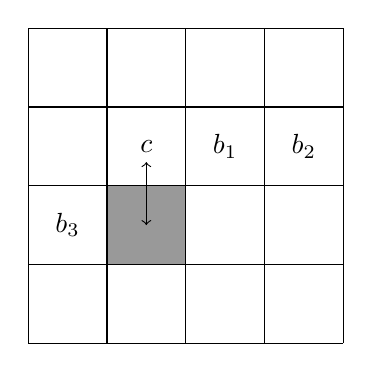
\begin{tikzpicture}
		\draw[step=1cm] (0, 0) grid (4, -4);
		\node()[anchor=center] at (0.5, -0.5) {};
		\node()[anchor=center] at (1.5, -0.5) {};
		\node()[anchor=center] at (2.5, -0.5) {};
		\node()[anchor=center] at (3.5, -0.5) {};
		%%%%%%%
		\node()[anchor=center] at (0.5, -1.5) {};
		\node(a)[anchor=center] at (1.5, -1.5) {$c$};
		\node()[anchor=center] at (2.5, -1.5) {$b_1$};
		\node()[anchor=center] at (3.5, -1.5) {$b_2$};
		%%%%%%%
		\node()[anchor=center] at (0.5, -2.5) {$b_3$};
		\node()[anchor=center] at (1.5, -2.5) {};
		\draw[fill=gray!80!white] (1,-2) rectangle (2, -3);
		\draw[<->] (a.south) -- (1.5,-2.5);
		\node()[anchor=center] at (2.5, -2.5) {};
		\node()[anchor=center] at (3.5, -2.5) {};
		%%%%%%%
		\node()[anchor=center] at (0.5, -3.5) {};
		\node()[anchor=center] at (1.5, -3.5) {};
		\node()[anchor=center] at (2.5, -3.5) {};
		\node()[anchor=center] at (3.5, -3.5) {};
		\end{tikzpicture}
	\end{center}
	
	From the above picture, the vertical move can be characterize as
	\begin{gather*}
		[(a_1, a_2, \ldots, c, b_1, b_2, b_3,\ldots ), (x,y)]\\
		\updownarrow\\
		[(a_1, a_2, \ldots, b_1, b_2, b_3,c, \ldots ), (x,y-1)]
	\end{gather*}
	
	That is this move skip an element($c$) over other 3 elements($b_1, b_2, b_3$) then change the row number by 1. (depending on the direction)
	
	After a magical moment one will have an idea that the invariant that is useful in this case is
	\[
		P(s) := n_\text{out of order pair} + y \text{ is even}
	\]
	where the number of out of order pair is, as the name said, the number of out of order pair. For example, for the follwing board
	\[
	t = [(1,2,3,4,7,8,9,10,5,6,11,12,13,14,15), (2,3)]
	\]
	The out of order pairs are (7,5), (7,6), (8,5), (8,6), (9,5), (9,6), (10,5), (10,6). 8 pairs in total and $y$ is 3. So, 8+3 is odd thus $P(t)$ is false.
	
	For the solved board, the number of out of order pairs is zero and y is 4. So, the sum is even.
	
	Now we have to prove that for every move the invariant is preserved. All we have to show is that the invariant is preserved for all moves.
	
	\theorem
		\[
		P(s) := n_\text{out of order pair} + y \text{ is even}
		\]
		is the perseved invairant.
		
	\proof
	Assuming that we start in the state $s_n$ where $P(s_n)$ is true. This means that the sum of the number of out of order pair and the row number is even.
	
	We want to show that the next state $s_{n+1}$ has the same property that is the sum of the number of out of order pair and the row number is even.
	
	The first case is horizontal move.
	
	For horizontal move.
	\begin{gather*}
	s_n = [ (a_1, a_2, \ldots, a_{15}), (x,y) ]\\
	\downarrow\\
	s_{n+1} = [ (a_1, a_2, \ldots, a_{15}), (x \pm 1,y) ]	\\
	\end{gather*}
	Since the order of the number stays the same. The number of out of order pair remains the same. Plus, the row number of blank spot doesn't change. The sum doesn't change. Therefore, the sum of the number of out of order pair and the row number is still even.
	
	For vertical move. The proof for the two cases of vertical move are the same so I will show here just one.
	\begin{gather*}
	s_n = [(a_1, a_2, \ldots, c, b_1, b_2, b_3,\ldots ), (x,y)]\\
	\downarrow\\
	s_{n+1}[(a_1, a_2, \ldots, b_1, b_2, b_3,c, \ldots ), (x,y-1)]
	\end{gather*}
	
	Let us consider the number of out of order pair which involve $c$ and one of, $b_1, b_2, b_3$. The number of out of order pair can be $0, 1, 2, 3$. After the move, the number of out of order pair will be come:
\begin{center}
		\begin{tabular}{|c|c|}
		\hline Before & After \\ 
		\hline  0 & 3 \\ 
		\hline  1 & 2 \\ 
		\hline  2 & 1 \\ 
		\hline  3 & 0 \\ 
		\hline 
	\end{tabular}
\end{center}
	
	This means that the number of out of order pair after the move flip the parity(odd to even and even to odd).
	
	The row also change by one. That means the row number also flip the parity.
	
	Since both numbers flip the parity, the sum remains even.
	
	Therefore, since both moves preserve the $P$.
	\[
	P(s) := n_\text{out of order pair} + y \text{ is even}
	\]
	is a preserved invaraint.
	\qedd.
	
	\collorary For the solved board, $P(\text{solved board})$ is true. 
	\begin{center}
		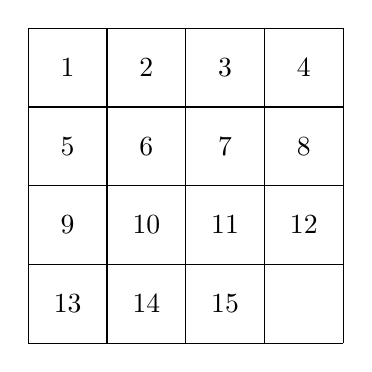
\begin{tikzpicture}
		\draw[step=1cm] (0, 0) grid (4, -4);
		\node()[anchor=center] at (0.5, -0.5) {1};
		\node()[anchor=center] at (0.5, -1.5) {5};
		\node()[anchor=center] at (0.5, -2.5) {9};
		\node()[anchor=center] at (0.5, -3.5) {13};
		\node()[anchor=center] at (1.5, -0.5) {2};
		\node()[anchor=center] at (1.5, -1.5) {6};
		\node()[anchor=center] at (1.5, -2.5) {10};
		\node()[anchor=center] at (1.5, -3.5) {14};
		\node()[anchor=center] at (2.5, -0.5) {3};
		\node()[anchor=center] at (2.5, -1.5) {7};
		\node()[anchor=center] at (2.5, -2.5) {11};
		\node()[anchor=center] at (2.5, -3.5) {15};
		\node()[anchor=center] at (3.5, -0.5) {4};
		\node()[anchor=center] at (3.5, -1.5) {8};
		\node()[anchor=center] at (3.5, -2.5) {12};
		\end{tikzpicture}
	\end{center}
	
	 But, for the switched board, $P(\text{flipped})$ is false. The flipped board is not reachable by vertical and horizontal moves.
	
	\begin{center}
		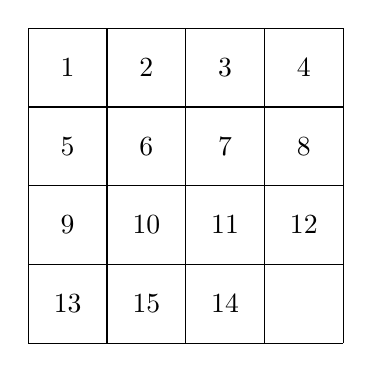
\begin{tikzpicture}
		\draw[step=1cm] (0, 0) grid (4, -4);
		\node()[anchor=center] at (0.5, -0.5) {1};
		\node()[anchor=center] at (1.5, -0.5) {2};
		\node()[anchor=center] at (2.5, -0.5) {3};
		\node()[anchor=center] at (3.5, -0.5) {4};
		\node()[anchor=center] at (0.5, -1.5) {5};
		\node()[anchor=center] at (1.5, -1.5) {6};
		\node()[anchor=center] at (2.5, -1.5) {7};
		\node()[anchor=center] at (3.5, -1.5) {8};
		\node()[anchor=center] at (0.5, -2.5) {9};
		\node()[anchor=center] at (1.5, -2.5) {10};
		\node()[anchor=center] at (2.5, -2.5) {11};
		\node()[anchor=center] at (3.5, -2.5) {12};
		\node()[anchor=center] at (0.5, -3.5) {13};
		\node()[anchor=center] at (1.5, -3.5) {15};
		\node()[anchor=center] at (2.5, -3.5) {14};
		\node()[anchor=center] at (3.5, -3.5) {};
		\end{tikzpicture}
	\end{center}
	\qedd
	
\end{enumerate}




\end{multicols}




\end{document}
